\documentclass{telkomnika}

%%required package. add for your convenient, but do not remove the initial
\setlength{\headsep}{0.15in}
\usepackage{amsmath, amsfonts, amssymb, float, fancyhdr}
\usepackage[figuresright]{rotating}
\usepackage{authblk, graphicx, indentfirst, lastpage, lipsum}
\usepackage{pifont}
\renewcommand{\Authsep}{, }
\renewcommand{\Authand}{, }
\renewcommand{\Authands}{, }
\setlength{\affilsep}{0cm}
\renewcommand\Authfont{\normalsize}
\renewcommand\Affilfont{\fontsize{8}{10}\mdseries}
\makeatletter
\renewcommand{\@biblabel}[1]{[#1]\hfill}
\renewcommand\AB@authnote[1]{\textsuperscript{\normalfont\bfseries#1}}
\makeatother
\usepackage[font=normalsize]{subfig, caption}
\usepackage{epstopdf}
\usepackage[left=3cm, right=2.5cm, top=2.5cm, bottom=2.5cm, includehead, includefoot]{geometry}
\usepackage[justification=centering]{caption}
\captionsetup{labelsep=period}
\usepackage{titlesec}
\usepackage{xcolor}
\titleformat{\section}
{\normalfont\normalsize\bfseries\uppercase}{\thesection}{1.7em}{}
\titleformat{\subsection}
{\normalfont\normalsize\bfseries}{\thesubsection}{.95em}{}
\titleformat{\subsubsection}
{\bfseries}{\thesubsubsection}{.2em}{}
\titlespacing*{\section}{0cm}{0.7cm}{0cm}
\usepackage{enumitem}
\usepackage[numbers,sort&compress]{natbib}
\usepackage{ragged2e}
\usepackage{hyperref,graphicx}
\usepackage{multirow}
\usepackage{url}
\usepackage{tikz}
\usetikzlibrary{3d}
\usetikzlibrary{automata,positioning}
\usepackage{tabularx}
\usepackage{booktabs}

%%leave copyright info to the editor
\CopyrightLine[]{}{\textit{This is an open access article under the \textcolor{blue}{\underline{CC BY-SA}} license.}
\vspace{.5em}}

%%author
\author[1]{\bfseries Kelvin*}
\author[1]{\bfseries Samuel Lukas}
%%author's affiliation
\affil[1]{Computer Science Department Faculty of Computer Science, Universitas Pelita Harapan,
UPH Tower, Lippo Karawaci, Tangerang, 15811, Indonesia}
\affil[*]{Corresponding author, e-mail: 01679220011@student.uph.edu, samuel.lukas@uph.edu}

%%title and shortitle (for footer)
\title{Mean End Analysis Decision Making Model in Santorini Board Game}
\shorttitle{Paper’s title should be the fewest possible words that accurately describe ... (First Author)}

%%starting
\begin{document}
\setcounter{page}{1}

%%indentation. do not change
\setlength{\parindent}{1.27cm}

%%header and footer setting. do not change
\pagestyle{fancy}
\fancyhfoffset{0cm}

%%journal info
\journalname{TELKOMNIKA Telecommunication, Computing, Electronics and Control}
\journalshortname{TELKOMNIKA Telecommun Comput El Control}
\journalhomepage{http://journal.uad.ac.id/index.php/TELKOMNIKA}
\vol{99}
\no{1}
\months{February}
\years{2099}
\issn{1693-6930}
\DOI{10.12928}
\pagefirst{1}
\pagelast{1x}
\IDpaper{paperID}


%%build title
\maketitle


%%border setting. do not change
\hrule
\vspace{.1em}
\hrule
\vspace{.5em}
\noindent
\parbox[t][][s]{0.315\textwidth}{%
\textbf{Article Info}
\vspace{.5em}
\hrule
\vspace{.5em}
\begin{history}
\vspace{.5em}

%%article info. editor's privilege
Received mm dd, yyyy

Revised mm dd, yyyy

Accepted mm dd, yyyy

\vspace{.7em}
\end{history}
\vspace{.5em}
\hrule
\vspace{.5em}
\begin{keyword} 
\vspace{.5em}
%%write keyword here. separate by \sep
First keyword \sep Second keyword \sep Third keyword \sep Fourth keyword \sep Fifth keyword
\vspace{.5em}
\end{keyword}
\vspace{\fill}
}
\parbox{0.020\textwidth}{\hspace{.5em}}
\parbox[t][][s]{0.65\textwidth}{%
\begin{abstract}
\vspace{.3em}
%% Text of abstract
This paper explores the use of Mean-End Analysis and heuristic functions to enhance AI in the board game Santorini, focusing on the strategic use of god powers like Apollo and Atlas. Traditional AI models have neglected these powers, limiting their effectiveness. Our research addresses this by developing an AI model that uses heuristic functions to make smarter decisions, significantly improving its strategic play. This not only demonstrates the AI's improved ability to navigate Santorini's complexities but also opens avenues for future work on AI strategy in games with changing dynamics, marking a notable contribution to AI and game strategy studies.
\end{abstract}
}
\parbox[l]{\textwidth}{%
\rule{0.275\textwidth}{0.5pt} \hspace{0.5cm} \hrulefill
\\
\emph{\textbf{Corresponding Author:}}
\vspace{.5em}\\
%% correspondence info. separate by \\
Kelvin\\
Computer Science Department Faculty of Computer Science, Universitas Pelita Harapan,\\
UPH Tower, Lippo Karawaci, Tangerang, 15811, Indonesia\\
Email: 01679220011@student.uph.edu
}
\vspace{.5em}
\hrule
\vspace{.1em}
\hrule


%% main text

\section{Introduction}
\label{}
The integration of artificial intelligence (AI) in board games has seen remarkable advancements, contributing significantly to the fields of game theory and computational intelligence. Santorini, a strategy board game renowned for its blend of simplicity and strategic depth, presents an interesting case study for AI research. Prior works, including Jack Boreham's exploration into developing an AI capable of playing Santorini, have focused on leveraging traditional AI techniques to navigate the game's complex decision spaces effectively. However, these studies predominantly target the game's basic mechanics, overlooking the nuanced strategic layers introduced by the god system \cite{Boreham2019}.

The god system in Santorini introduces unique powers and abilities, significantly diversifying gameplay and strategic considerations. This aspect of Santorini has been underexplored in AI research, representing a gap in our understanding of AI's potential to adapt to and leverage variable player powers in board games. Boreham's project, while providing a solid foundation in AI development for Santorini, does not delve into the complexities introduced by the god system, focusing instead on a basic version of the game \cite{Boreham2019}.This gap highlights a broader trend in AI board game research, where the variability and strategic depth added by such systems are often overlooked.

This research aims to fill this gap by focusing on the integration of Mean End Analysis and heuristic functions to address the unique challenges posed by the god system in Santorini. By doing so, it seeks not only to enhance AI performance in a more complex version of Santorini but also to contribute to the broader discourse on AI adaptability in board games featuring variable player powers. Through a critical analysis of existing AI strategies, as illustrated by Boreham's work, and the development of novel MCTS adaptations, this research aims to illuminate AI potential in navigating variable player powers introduced by Santorini's god system \cite{Boreham2019}.



\section{Method}
\label{}
Explaining research chronological, including research design, research procedure (in the form of algorithms, Pseudocode or other), how to test and data acquisition [5]–[7]. The description of the course of research should be supported references, so the explanation can be accepted scientifically [2], [4]. Figures 1-2 and Table 1 are presented center, as shown below and cited in the manuscript [5], [8]–[13]. The nodes energy consumption in network OHCRP (50\%\ DSr) vs SPEED has been illustrated in Figure 2(a) and network OHCRP (50% DSr) vs THVR has been illustrated Figure 2(b).
\subsection{Game State Design}
A game state refers to a digital snapshot of all relevant information in a game at any given moment, encompassing the position of pieces, the current player's turn, and any other pertinent data that defines the game's status \cite{Jarvinen2008}. The game state is a structured representation that breaks down the game into manageable components, each reflecting an a aspect of gameplay, the game state is segmented into six elements:
\begin{enumerate}
    \item \textbf{Current Player's Turn:} Identifies which player's turn it is to act, represented by a single value string, such as "p1" or "p2", indicating the active player.
    \item \textbf{State Action:} Current action phase of state within a player's turn: "pick god", "place worker", "move", "build", along with outcomes like "win", "lose", and "draw".
    \item \textbf{Active Worker:} Which worker is currently engaged for the player, denoted by identifiers such as "w1" or "w2". This specification is crucial for building, which necessitate knowledge of the worker's id after moving.
    \item \textbf{Players and Their Gods:} Lists the players along with the gods they have chosen, such as \texttt{[['p1', 'Atlas'], ['p2', 'Apollo']]}.
    \item \textbf{Building Board:} This component represents the levels of construction on the board, with numbers from 0 to 4, where '0' indicates an empty tile, '1' to '3' represent the height of buildings, and '4' denotes a dome. This model simplifies the representation by standardly using '4' for domes, although, in practice, the god power of Atlas allows for the placement of domes at any level.
    \item \textbf{Worker Board:} This component represents positions of workers using designations like "p1w1" for Player 1's first worker.
\end{enumerate}
\begin{figure}[!ht]
\centering
\(S = 
\left[
    \begin{array}{l}
        \text{'p2'}, \\
        \text{`move'}, \\
        \text{`'}, \\
        \left[ \begin{array}{ll} \text{'p1'} & \text{'Atlas'} \\ \text{'p2'} & \text{'Apollo'} \end{array} \right], \\
        \left[ 
    \begin{array}{ccccc} 
        1 & 2 & 3 & 4 & 2 \\
        0 & 1 & 1 & 1 & 1 \\
        0 & 1 & 1 & 1 & 0 \\
        0 & 0 & 0 & 0 & 0 \\
        0 & 0 & 0 & 0 & 0
    \end{array}\right], \\
    \left[ 
        \begin{array}{ccccc} 
            \text{''} & \text{'p1w1'} & \text{''} & \text{''} & \text{''} \\ 
            \text{''} & \text{'p2w2'} & \text{''} & \text{''} & \text{''} \\ 
            \text{'p1w2'} & \text{''} & \text{''} & \text{''} & \text{''} \\ 
            \text{''} & \text{''} & \text{''} & \text{''} & \text{''} \\ 
            \text{'p2w1'} & \text{''} & \text{''} & \text{''} & \text{''}
        \end{array} \right]
\end{array}
\right]\)\par
\caption{Example of a game state}
\label{fig:game-state}
\end{figure}

As depicted in Figure.~\ref{fig:game-state}, this game state representation designed for Santorini, while comprehensive and structured, is primarily tailored for human readability and understanding. It intuitively segments the game into distinct elements. However, for the purposes of machine learning and AI strategy development, this representation usually is transformed into a format conducive to computational processing. In the scope of this research, no transformation is done for simplicity. The representation remains in its original form, maintaining its human-readable structure without conversion into numerical values or one-hot encoding techniques.

\subsection{Game Engine Design}
Historically, game engines have been developed as software frameworks aimed at facilitating video game creation and development. These engines typically feature several key elements, such as a rendering engine (also known as a "renderer") that supports both 2D and 3D graphics, a physics engine for managing collision detection and its outcomes, and a scene graph that oversees the handling of models, scripts, audio, threading, and networking, among other functionalities \cite{Wang2018}. In the case of the Santorini board game, the game engine calculates possible moves players can make from given game state and then updates the game accordingly. This means it compute all allowed moves, calculate and changes the game's current state based on those moves. 
\begin{figure}[!ht]
\centering
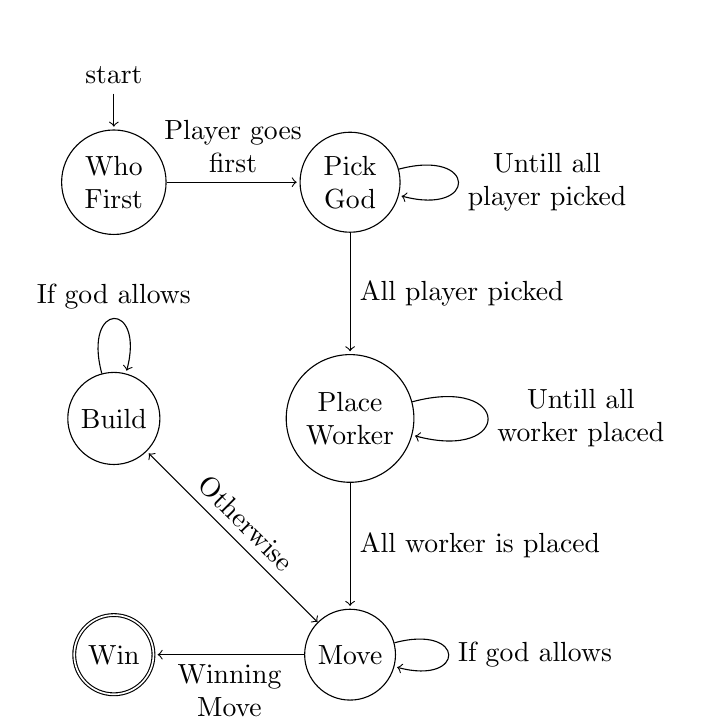
\begin{tikzpicture}[shorten >=1pt,node distance=3cm,on grid,auto] 
    \node[state,initial, initial where=above, align=center] (choose)   {Who\\First}; 
    \node[state] (pick) [right=of choose, align=center] {Pick\\God}; 
    \node[state] (place) [below=of pick,align=center] {Place\\Worker}; 
    \node[state] (move) [below=of place] {Move}; 
    \node[state] (build) [left=of place] {Build}; 
    \node[state,accepting](win) [left=of move] {Win};
 
    \path[->] 
    (choose) edge [align=center] node {Player goes\\first}(pick)
    (pick) edge [loop right, align=center] node {Untill all\\player picked} (pick)
    (pick) edge node {All player picked} (place)
    (place) edge [loop right, align=center] node {Untill all\\worker placed} (place)
    (place) edge node {All worker is placed} (move)
    (move) edge [loop right, align=center] node {If god allows} (move)
    (move) edge[<->] [align=center, sloped] node {Otherwise} (build)
    (move) edge [align=center] node {Winning\\Move} (win)
    (build) edge [loop above, align=center] node {If god allows} (build);

\end{tikzpicture}
\caption{Finite State Machine representing the game process.}
\label{fig:game-fsm}
\end{figure}

The game engine describe the flow of the game through a series of states, 
as illustrated by the finite state machine (FSM) in Figure.~\ref{fig:game-fsm}. 
FSM are utilized to model strategies in extensive-form games, where each machine represents a set of actions and transitions dictated by the game's outcomes\cite{Cerny2020}.  
The process begins with the initial state "Who First", where the system determines the order of play. 
Upon establishing the first player, the game transitions into the "Pick God" state. 
Here, players sequentially select their gods, each providing unique abilities or advantages. 
This selection process is iterative, denoted by the loop back to the same state, and continues until all players have made their choices.

After the selection phase, the game progresses to the "Place Worker" state, where players place their 2 workers on the board. Similar to the god selection, this phase is also iterative and continues until all participants have placed their workers, The iterative nature of this state ensures that the setup is complete and follows the game rule before moving forward. The "Move" state follows, representing the core of the game's mechanics where players move their workers around the board. This state has multiple outcomes: it can loop back to itself if the chosen god's powers allow for additional movement; it can transition to the "Build" state, allowing the player to construct buildings or structures; or it can lead to the "Win" state if the move satisfies the winning conditions.

In the "Build" state, players build structures which are pivotal for progressing in the game. This state, similar to "Move", can loop back on itself if the player's god permits additional building actions. The game transitions back to the "Move" state. The "Win" state signifies the end of the game.As depicted in Figure.~\ref{fig:game-fsm}, each of the game states (Who First, Pick God, Place Worker, Move, Build, and Win) updates the game state from the example state Figure.~\ref{fig:game-state}. In particular, the 'Who First' state decides which player starts the game, affecting the 'p1' and 'p2' in the first element of the list. The 'Pick God' state assigns gods to each player, influencing the god assignments in the fourth element of the list which is player god list. As players place their workers ('Place Worker') and move them ('Move'), this is reflected in the worker positions within the game board list on the sixth element. 
Finally, 'Build' actions alter the board layout on the fifth element.
The four actions: pick god, place worker, move, and build is then categorized as operators, 
each with specific preconditions and results. 

From the sample game state and flow state diagram provided, a mathematical model for Santorini board game is constructed.With limitation of focusing solely on the gods Apollo and Atlas in the mathematical model provides a concise framework to illustrate how heuristic values can influence the use of god powers effectively within AI strategies. This constraint, while reducing the game's complexity, offers a clear perspective on how specific god powers can be leveraged and optimized through heuristic evaluation, 
demonstrating the impact of these powers on strategic decision-making in a controlled setting.

\subsection{Game State and Game Engine Mathematical Model}
First, define the number of players, \(n\), such that \(2 \leq n \leq 4\). Then, construct the player and worker set \( \text{Players} = \{p_1, p_2, \ldots, p_n\} \),\(\text{Workers} = \{p_{1}w_{1},p_{1}w_{2},p_{2}w_{1},p_{2}w_{2}, \ldots, p_{n}w_{1},p_{n}w_{2}\}\) Define the set of gods as \(\text{Gods} = \{\text{"Atlas"}, \text{"Apollo"}\}\).Then the turn action set which defines what action is available \(\text{TurnAction} = \{\text{"pick god"}, \text{"place worker"}, \text{"move"}, \text{"build"}\}\).From that we can construct state tuple as \(S_t = (\text{CPlayer}, \text{Phase}, \text{AWrk}, \text{PGods}, \text{Building}, \text{Worker})\).With each element criteria as \(\text{CPlayer} \in \text{Players}\),\(\text{Phase} \in \text{TurnAction}\),\(\text{ActiveWorker} \in \text{Workers} \text{ if and only if } \text{Phase} = \text{"build"}\), \(PGods\) as seen in Equation~\ref{eq:playergods},\(Building\) as seen in Equation~\ref{eq:board_build}, and \(Worker\) as seen in Equation~\ref{eq:board_worker}.

\begin{equation}
    \begin{aligned}
    \text{PGods} = \begin{bmatrix}
    p_1 & \text{god}_1 \\
    p_2 & \text{god}_2 \\
    \vdots & \vdots \\
    p_n & \text{god}_n \\
    \end{bmatrix}\\
    p_i \in \text{Players} \land \text{god}_i \in \text{Gods}
    \end{aligned}
    \label{eq:playergods}
\end{equation}
\begin{equation}
    \begin{aligned}
    \text{Building} = \begin{bmatrix}
    b_{11} & b_{12} & b_{13} & b_{14} & b_{15} \\
    b_{21} & b_{22} & b_{23} & b_{24} & b_{25} \\
    b_{31} & b_{32} & b_{33} & b_{34} & b_{35} \\
    b_{41} & b_{42} & b_{43} & b_{44} & b_{45} \\
    b_{51} & b_{52} & b_{53} & b_{54} & b_{55} \\
    \end{bmatrix}\\
    \forall i,j \in \{1,2,3,4,5\}, 0 \leq b_{ij} \leq 4
    \end{aligned}
    \label{eq:board_build} 
\end{equation}

\begin{equation}
    \begin{aligned}
    \text{Worker} = \begin{bmatrix}
    w_{11} & w_{12} & w_{13} & w_{14} & w_{15} \\
    w_{21} & w_{22} & w_{23} & w_{24} & w_{25} \\
    w_{31} & w_{32} & w_{33} & w_{34} & w_{35} \\
    w_{41} & w_{42} & w_{43} & w_{44} & w_{45} \\
    w_{51} & w_{52} & w_{53} & w_{54} & w_{55} \\
    \end{bmatrix}\\
    \forall i,j \in \{1,2,3,4,5\}, 0 \leq w_{ij} \leq 4
    \end{aligned}
    \label{eq:board_worker} 
\end{equation}

From these criteria, we can construct an operator table as shown in Table~\ref{tab:operators} that facilitates interaction with the game state through specific operators.
Each operator is associated with a set of predefined conditions and, when applied, transitions the game into a new state, enabling continued gameplay.

\begin{table}[h]
\caption{Operators for Santorini Game}
\label{tab:operators}
\begin{tabularx}{\textwidth}{|X|X|X|}
\hline
\textbf{Operator} & \textbf{Precondition} & \textbf{Results} \\ \hline
OP(1): Generate Starting State \newline genStart(n, p) & 
$2 \leq n \leq 4 \land n \in \mathbb{Z}$ \newline $p \in \text{Players}$ & 
$S_0 = \{CPlayer, Phase,$
$ActiveWorker, PGods,\}$
$BBuild, BWorker\}$ \newline
$S_0 \gets \text{Equation~\ref{eq:start_state}}(n, p)$ \\ \hline
OP(2): Pick God \newline pickGod$(S_t, \text{god})$ & 
$S_t[1] = \text{'pick god'}$ \newline $\text{god} \in \text{Gods}$ & 
$S_{t+1} \gets \text{Equation~\ref{eq:pick_god}}(S_t, \text{god})$ \\ \hline
OP(3): Place Worker \newline placeWorker$(S_t, i_1, j_1, i_2, j_2)$ & 
$S_t[1] = \text{'place worker'}$ \newline $\neg(i_1 = i_2 \land j_1 = j_2)$ \newline $\forall a \in \{i_1, j_1, i_2, j_2\}, 0 \leq a \leq 4$ \newline $S_t[5][i_1][j_1] = \emptyset$ \newline $S_t[5][i_2][j_2] = \emptyset$ & 
$S_{t+1} \gets \text{Equation~\ref{eq:place_worker}}(S_t, i_1, j_1, i_2, j_2)$ \\ \hline
OP(4): Move \newline moveWorker$(S_t, p_xw_y, i, j)$ & 
$S_t[1] = \text{'move'}$ \newline $1 \leq x \leq n$ \newline $1 \leq y \leq 2$ \newline $\forall a \in \{i, j\}, 0 \leq a \leq 4$ \newline
Equation~\ref{eq:chk_worker_pos} \newline
if $god_{st[0]} =  \text{'Appolo'}$\newline
$then \text{ Equation~\ref{eq:chk_worker_move}}$
$otherwise \text{ Equation~\ref{eq:chk_worker_appolo}}$& 
$S_{t+1} \gets \text{Equation~\ref{eq:worker_move}}(S_t, p_xw_y, i, j)$ \\ \hline
OP(5): Build \newline buildWorker$(S_t, p_xw_y, i, j, d)$ & 
$S_t[1] = \text{'build'}$ \newline $1 \leq x \leq n$ \newline $1 \leq y \leq 2$ \newline $\forall a \in \{i, j\}, 0 \leq a \leq 4$ \newline
Equation~\ref{eq:chk_worker_pos}\newline 
$\neg (\text{{god}}_{S_t[0]} \neq \text{'Atlas'} \land d = \text{True})$\newline
Equation~\ref{eq:chk_worker_pos} & 
$S_{t+1} \gets \text{Equation~\ref{eq:worker_build}}(S_t, p_xw_y, i, j, d)$ \\ \hline
\end{tabularx}
\end{table}

The operator \( \text{OP}(1): \text{GenerateStartingState} \) as shown by Table~\ref{tab:operators}, represented by \( \text{genStart}(n, p) \) and showcased in Equation~\ref{eq:start_state}, shows the process for generating the initial game state \( S_0 \). This state is structured into components for setup: \( S_0[0] \) is set to player \( p \), marking the starting player; \( S_0[1] \) is assigned the action 'pick god', indicating the initial action to be taken; \( S_0[2] \) is initialized as \( \emptyset \), representing an empty set for the active worker during the build phase. For each player \( i \) in the range from 1 to \( n \), \( S_0[3] \) initializes each player's god \( \text{god}_i \) as \( \emptyset \), signifying no god selection at the start. Additionally, \( S_0[4] \) and \( S_0[5] \) for each cell in a 5x5 grid are set to 0 for no building and \( \emptyset \) for no worker, respectively, preparing the board with default values and empty slots, thus laying the groundwork for game progression from this initial configuration.

\begin{equation}
    \begin{aligned}
        S_0[0] &\leftarrow p \\
        S_0[1] &\leftarrow \text{"pick god"} \\
        S_0[2] &\leftarrow \emptyset \\
        \forall i \in \{1, 2, \ldots, n\}, S_{0}[3]\text{god}_i &\leftarrow \emptyset \\
        \forall i,j \in \{1,2,3,4,5\}, S_{0}[4]b_{ij} &\leftarrow 0 \\
        \forall i,j \in \{1,2,3,4,5\}, S_{0}[5]w_{ij} &\leftarrow \emptyset
    \end{aligned}
    \label{eq:start_state}
\end{equation}

Following the initial state setup, the operator \( \text{OP}(2): \text{PickGod} \) advances the game into its next state as specified by Equation~\ref{eq:pick_god}. This equation assigns a specific god to a player based on the input god. Once all gods have been selected, indicating each \( \text{god}_i \neq \emptyset \) for \( i \) ranging from 1 to \( n \), the game action phase transitions to 'place worker', indicating a shift in gameplay dynamics. Concurrently, Equation~\ref{eq:next_player} is invoked to advance the turn to the next player. Specifically, if the current player \( S_t[0] \) is equal to \( S_t[3]_{pi} \), and \( i = n \), indicating the last player, then \( S_t[0] \) is reset to \( p_1 \), the first player, to maintain the turn cycle. Otherwise, the turn shifts to \( p_{i+1} \), the next sequential player. This mechanism ensures a smooth transition of turns among players following the god selection phase, systematically moving the game forward by updating player turns and transitioning into new phases of gameplay.

\begin{equation}
\label{eq:next_player}
\forall i \in \{1, 2, \ldots, n\}, \quad \text{if } S_t[0] = S_t[3]{pi}, \text{ then if } i=n \text{ then } S_t[0] \leftarrow p_1, \text{ otherwise } S_t[0] \leftarrow p_{i+1}
\end{equation}

\begin{equation}
    \begin{aligned}
        &\forall i \in \{1,2,\ldots, n\}, \text{ if } S_t[0] = S_t[3]p_i, \text{ then } S_t[3]\text{god}_i \leftarrow \text{god}\\
        &\text{if }\forall i \in \{1,2,\dots,n\}, \bigwedge \text{god}_i \neq \emptyset,\text{then} S_0[1] \leftarrow \text{"place worker"}\\
        &\text{Call Equation~\ref{eq:next_player}}
    \end{aligned}
    \label{eq:pick_god}
\end{equation}

The ``PlaceWorker'' operator, denoted by \( \text{OP}(3):\text{PlaceWorker} \) as shown on Table~\ref{tab:operators} and executed as \( \text{placeWorker}(S_t, i_1, j_1, i_2, j_2) \), outlines the prerequisites for placing workers on the game board within the 'place worker' phase. Firstly, the game state \( S_t[1] \) must explicitly be in the 'place worker' phase, ensuring that the action to place workers is timely and relevant. The operator also mandates that the positions designated for the two workers, marked by coordinates \( (i_1, j_1) \) and \( (i_2, j_2) \), must be distinct, preventing the allocation of both workers to the same location on the board. Additionally, these coordinates must fall within the board's confines, specified by a range from 0 to 4, to guarantee the placements are valid. Finally, the targeted positions for the workers, identified by \( S_t[5][i_1][j_1] \) and \( S_t[5][i_2][j_2] \) are required to be vacant (\(\emptyset\)), confirming that the selected spots are free for worker placement. By satisfying these criteria, the ``PlaceWorker'' operator effectively places a player's workers on the game board, thereby updating the game's state to reflect the new board configuration and advancing the gameplay accordingly.

\begin{equation}
    \begin{aligned}
        &S_t[5][i_1][j_1] \leftarrow S_t[0] w_1 \\
        &S_t[5][i_2][j_2] \leftarrow S_t[0] w_2 \\
        &\text{if}\left ( \sum_{i=1}^{5}\sum_{j=1}^{5}\text{if } S_t[5][i][j]\neq \emptyset,\text{then } 1, \text{otherwise } 0 \right )=2n \\
        &\text{then } S_t[1] \leftarrow \text{"move"}\\
        &\text{Call Equation~\ref{eq:next_player}}
    \end{aligned}
    \label{eq:place_worker}
\end{equation}

Once the conditions for the ``PlaceWorker'' operation are fulfilled, the game progresses to execute Equation ~\ref{eq:place_worker}, applying the operation \( \text{placeWorker}(S_t, i_1, j_1, i_2, j_2) \) to advance the game state to \( S_{t+1} \). This equation is pivotal for physically placing the workers on the board: \( S_t[5][i_1][j_1] \) is updated to hold the first worker \( w_1 \), associated with the current player \( S_t[0] \) (for example, ‘p1w1’), and similarly, \( S_t[5][i_2][j_2] \) is updated to contain the second worker \( w_2 \). Following the placement, the game checks if all players have positioned their workers by evaluating whether the total number of occupied spots on the board equals \( 2n \), where \( n \) represents the number of players. If this condition is met, indicating that each player has placed their two workers, the game phase shifts to 'move' as \( S_t[1] \) is updated to 'move'. Consequently, Equation~\ref{eq:next_player} is invoked to transition the game to the next player, thereby ensuring the game's flow continues seamlessly from worker placement to the next player or phase of gameplay.

\begin{equation}
\bigwedge\forall w_i, w_j \in \{0,1,2,3,4\},\text{if } S_t[5][w_i][w_j] = p_x w_y 
    \text{ then } \neg(w_i=i \land w_j=j) \text{ otherwise True}
    \label{eq:chk_worker_pos}
\end{equation}

\begin{equation}
 \begin{aligned}
    &\forall w_i, w_j \in \{0,1,2,3,4\},\text{if } S_t[5][w_i][w_j] = p_x w_y \text{ then break}\\
    &S_t[5][i][j]=\emptyset \land S_t[4][i][j]\neq 4 \land |w_i-i|\leq 1 \land |w_j-j| \leq 1 \land\\
    &(S_t[4][w_i][w_j]+1=S_t[4][i][j] \vee S_t[4][w_i][w_j] \geq S_t[4][i][j] )\\
 \end{aligned}
\label{eq:chk_worker_move}
\end{equation}

\begin{equation}
 \begin{aligned}
    &\forall w_i, w_j \in \{0,1,2,3,4\},\text{if } S_t[5][w_i][w_j] = p_x w_y \text{ then break}\\
    &S_t[5][i][j]\notin \{p_xw_1,p_xw_2\} \land S_t[4][i][j]\neq 4 \land |w_i-i|\leq 1 \land |w_j-j| \leq 1 \land\\
    &(S_t[4][w_i][w_j]+1=S_t[4][i][j] \vee S_t[4][w_i][w_j] \geq S_t[4][i][j] )\\
 \end{aligned}
\label{eq:chk_worker_appolo}
\end{equation}

The ``Move'' operator, \( \text{OP}(4):\text{Move} \), detailed as \( \text{moveWorker}(S_t, p_xw_y, i, j) \), outlines the requirements for moving a worker on the game board. This operation is permissible only when the game is in the 'move' phase, as indicated by \( S_t[1] = \text{'move'} \). The conditions specify that \( x \), denoting the player number, must be within the range of 1 to \( n \), where \( n \) is the total number of players, and \( y \), representing one of the two workers for each player, must be either 1 or 2. Furthermore, the destination coordinates \( (i, j) \) must lie within the 5x5 grid, hence \( \forall a \in \{i, j\}, 0 \leq a \leq 4 \). Equation ~\ref{eq:chk_worker_pos} sets the precondition that the intended move should not place a worker on a cell that is already occupied by the same worker, ensuring movement occurs. The specifics of the move depend on the current player's god ability. If the player's god is 'Apollo', Equation  ~\ref{eq:chk_worker_appolo} is applied; otherwise, Equation  ~\ref{eq:chk_worker_move} governs the move. The distinction between the conditions set forth in Equations  ~\ref{eq:chk_worker_move} and ~\ref{eq:chk_worker_appolo} for the "Move" operator revolves around the handling of occupied tiles. While both conditions prohibit moving to a tile occupied by a level 4 block that is a dome \(( S_t[4][i][j] \neq 4 )\), ensuring the move is within one space \( (\left| w_i - i \right| \leq 1 \land \left| w_j - j \right| \leq 1 ) \), and adhering to movement to a space of equal or one level higher than the worker's current position, the crucial difference lies in their approach to occupied tiles. Specifically, Equation ~\ref{eq:chk_worker_move} requires the destination tile \( S_t[5][i][j] \) to be unoccupied \( (\emptyset) \), catering to standard movement rules. Conversely, Equation ~\ref{eq:chk_worker_appolo}, applicable when the player's god is 'Apollo', allows for the swapping of positions with another player's worker, provided the destination tile does not contain one of the moving player's own workers \( (S_t[5][i][j] \notin \{p_xw_1, p_xw_2\}) \). This nuanced approach introduces a strategic layer for players with the 'Apollo' god power, allowing them to interact with other players' workers on the board, thus enriching the tactical depth and complexity of the movement phase while upholding the integrity and competitive balance of the gameplay.

\begin{equation}
 \begin{aligned}
    &\forall w_i, w_j \in \{0,1,2,3,4\},\text{if } S_t[5][w_i][w_j] = p_x w_y \text{ then break}\\
    &w_t \leftarrow S_t[5][i][j]\\
    &S_t[5][w_i][w_j]\leftarrow S_t[5][i][j]\\
    &S_t[5][i][j] \leftarrow w_t \\
    &\text{if } S_t[4][i][j]=3\text{ then } S_t[1] \leftarrow \text{"win"}\\
    &\text{otherwise } (S_t[1] \leftarrow \text{"build" Call Equation~\ref{eq:next_player}})
 \end{aligned}
\label{eq:worker_move}
\end{equation}

Once the preconditions for the ``Move'' operation are satisfied, Equation Equation ~\ref{eq:worker_move} is invoked to generate the next state of the worker's move to the new position, transitioning the game state to \( S_{t+1} \). This equation plays a crucial role in updating the board's configuration: if a worker identified as \( p_xw_y \) occupies a tile \( (w_i, w_j) \), the operation swaps the worker's current position with the targeted position \( (i, j) \). Specifically, \( w_t \), which temporarily holds the worker's identifier, facilitates the exchange by first capturing the worker at \( (w_i, w_j) \), then updating the tile \( (w_i, w_j) \) with the content of the destination tile \( (i, j) \), and finally setting the destination tile with \( w_t \) value. The distinction between Apollo's ability and that of other gods becomes irrelevant in this context, as the mechanics of swapping are consistent: Apollo's power allows for swapping with another player's worker, whereas, for other gods, the swap is essentially with an empty tile. Therefore, the procedural outcome remains the same, facilitating the worker's relocation on the board.

Furthermore, if the destination tile \( (i, j) \) has a building height of 3 \( (S_t[4][i][j] = 3) \), it triggers a win condition, updating \( S_t[1] \) to 'win'. Otherwise, the game progresses to the 'build' phase, and Equation ~\ref{eq:next_player} is called to advance the turn to the next player. This sequential process not only orchestrates the worker's movement but also integrates the possibility of achieving a win condition based on the movement's outcome, thereby seamlessly transitioning into the subsequent game phase or concluding the game with a victory.

    
\begin{equation}
 \begin{aligned}
    &\forall w_i, w_j \in \{0,1,2,3,4\},\text{if } S_t[5][w_i][w_j] = p_x w_y \text{ then break}\\
    &S_t[5][i][j]=\emptyset \land S_t[4][i][j]\neq 4 \land |w_i-i|\leq 1 \land |w_j-j| \leq 1 \land\\
 \end{aligned}
\label{eq:chk_worker_build}
\end{equation}

The ``Build'' operator, denoted as \( \text{OP}(5):\text{Build} \) which is done after the action ``move'' defined by the equation from Table ~\ref{tab:operators} \( \text{buildWorker}(S_t, p_xw_y, i, j, d) \), sets forth the criteria necessary for executing a building action on the game board. This operator is activated during the 'build' phase, indicated by \( S_t[1] = \text{'build'} \), and is designed to adjust the board's structure by either adding a level to a building or, in the case of the god Atlas, placing a dome. Key prerequisites for this operator encompass: confirmation that the game is within the 'build' phase; validation that the player number \( x \) falls within the 1 to \( n \) range, with \( n \) representing the total player count; assurance that the worker identifier \( y \) is either 1 or 2, linking to one of the player's workers; and verification that the targeted coordinates \( (i, j) \) for the building activity are confined within the grid limits of 0 to 4. Additionally, adherence to Equation ~\ref{eq:chk_worker_pos} is necessitated, verifying that the target tile is not the worker's current location, thus ensuring a logical and valid move. Moreover, the specific inclusion of Equation ~\ref{eq:chk_worker_build} introduces a further constraint, mandating the target tile for construction to be unoccupied \( (S_t[5][i][j] = \emptyset) \) and not capped by a level 4 dome \( (S_t[4][i][j] \neq 4) \), with the build location being within one space of the worker's position. This condition aligns with the strategic elements of the game, dictating the spatial dynamics of building actions. An additional layer of complexity is provided by the special condition for Atlas's ability, permitting dome placement at any construction phase when \( d \) is True, unless Atlas is not the current god in play, thus disallowing the dome action.

\begin{equation}
 \begin{aligned}
    &\text{if } d = True \text{ then }S_t[4][i][j]\leftarrow 4\\
    &\text{otherwise } S_t[4][i][j] \leftarrow S_t[4][i][j]+1\\
    &S_t[1]\leftarrow \text{"move"}\\
    &\text{Call Equation~\ref{eq:next_player}}
 \end{aligned}
\label{eq:worker_build}
\end{equation}

Upon meeting the set preconditions, the ``Build'' operation progresses to invoke Equation ~\ref{eq:worker_build}, which is articulated as \( S_{t+1} \gets \text{Equation ~\ref{eq:worker_build}}(S_t, p_xw_y, i, j, d) \). This equation finely tunes the building mechanics, especially taking into account the god power of Atlas. When the condition \( \neg (\text{god}_{S_t[0]} \neq \text{'Atlas'} \land d = \text{True})\) is fulfilled, the building action diverges based on the boolean value of \( d \). If \( d \) equals True, indicating the intention to use Atlas's power to place a dome, the building height at the targeted coordinates \((i, j)\) is directly set to 4, symbolizing the placement of a dome irrespective of the current building level. Conversely, if \( d \) is False, reflecting a standard building action, the building height at \((i, j)\) is incremented by one, following normal game rules for construction. Subsequently, the game phase is updated to 'move', and Equation ~\ref{eq:next_player} is called to transition the turn to the next player. This sequence ensures that after a building action is completed, whether it involves escalating a building's height or placing a dome by invoking the special ability of Atlas, the game fluidly moves forward, shifting the active phase back to player movement. 

The defined operators and their preconditions are essential for the game engine's operation, orchestrating the sequence of gameplay phases and ensuring adherence to the game's strategic and rule-based structure. With this foundation in place, the next critical step is to develop a heuristic function. This function will assess potential moves by assigning values to game states, guiding players in identifying the most advantageous actions. This progression from establishing game mechanics to integrating a decision-making framework is pivotal in enhancing the game's strategic depth and optimizing gameplay outcomes.

\subsection{Heuristic Function}

This research defines heuristic values from 0 to 100 for AI decision-making in the move and build phases, based on operator Table~\ref{tab:operators} preconditions. A value of 100 indicates actions that ensure a win. Additionally, using god powers rewards higher heuristic value, motivating the AI to utilize these abilities for strategic advantage. This approach aims to refine AI tactics by encouraging the use of god powers and prioritizing actions that significantly impact game outcomes.

\subsubsection {Move Heuristic Function}
\begin{equation}
 \begin{aligned}
    &\max(\forall i,j \in \{0, 1, 2, 3, 4\}, \forall y \in \{1, 2\},\text{if } \text{moveWorker}(S_t, S_t[0][w_y], i, j) = \text{True} \text{ then if } \\
    &\text{god}_{S_t[0]} = \text{'Apollo'} \text{ then } f_{\text{Apollo}}(S_t, i, j) \text{ otherwise } f_{\text{move}}(S_t, i, j) )
 \end{aligned}
\label{eq:move_max_heur}
\end{equation}

\begin{equation}
 \begin{aligned}
    &\mathbf{f}_{\text{move}}(\mathbf{S}, \mathbf{i}, \mathbf{j}) = \left\{
\begin{array}{cl}
100 & \text{if } \mathbf{S}[4][\mathbf{i}][\mathbf{j}] = 3 \\
5 & \text{if } \mathbf{S}[4][\mathbf{i}][\mathbf{j}] = 2 \\
2 & \text{if } \mathbf{S}[4][\mathbf{i}][\mathbf{j}] = 1 \\
1 & \text{if } \mathbf{S}[4][\mathbf{i}][\mathbf{j}] = 0 \\
\end{array}
\right.\\
 \end{aligned}
\label{eq:move_norm_heur}
\end{equation}

\begin{equation}
\mathbf{f}_{\text{Apollo}}(\mathbf{S}, \mathbf{i}, \mathbf{j}) = \left\{
\begin{array}{cl}
100 & \text{if } \mathbf{S}[4][\mathbf{i}][\mathbf{j}] = 3 \\
10 & \text{if } \mathbf{S}[4][\mathbf{i}][\mathbf{j}] = 2 \\
5 & \text{if } \mathbf{S}[4][\mathbf{i}][\mathbf{j}] = 1 \\
1 & \text{if } \mathbf{S}[4][\mathbf{i}][\mathbf{j}] = 0 \\
\end{array}
\right. \text{if } \mathbf{S}[5][\mathbf{i}][\mathbf{j}] \notin \{\mathbf{S}[0]w_1, \mathbf{S}[0]w_2, \emptyset\}
\text{ otherwise }
\mathbf{f}_{\text{move}}(\mathbf{S}, \mathbf{i}, \mathbf{j})
\label{eq:move_appolo_heur}
\end{equation}

The move heuristic function as shown in Equation ~\ref{eq:move_max_heur} aims to calculate the optimal move by calculating the maximum heuristic value among all valid moves for a game state \( S \), considering all possible positions \( i, j \) on the 5x5 board and each player's two workers \( y \). Validity is determined by whether a move action \( \text{moveWorker}(S_t, S_t[0]w_y, i, j) \) is possible. If a move is valid, its value is assessed based on whether the player's god is 'Apollo' and the specific conditions met at the target location. For non-'Apollo' moves, the heuristic values are assigned as follows as shown in Equation ~\ref{eq:move_norm_heur}: moving to a level 3 tile scores 100, indicating a win; a level 2 tile scores 5; a level 1 tile scores 2; and a ground-level tile scores 1. This tiered system prioritizes moves that lead closer to victory or offer strategic positioning. For 'Apollo' moves, the heuristic values are enhanced if the target tile is not occupied by the player's workers or is empty as shown in Equation ~\ref{eq:move_appolo_heur}: 100 for level 3 (winning move), 10 for level 2, 5 for level 1, and 1 for ground level. This increase reflects 'Apollo's ability to swap places with an opponent's worker, providing strategic advantages like swapping with opponent positioning for a win. If a move does not meet the 'Apollo' criteria, it defaults to the standard move valuation. This heuristic function Equation ~\ref{eq:move_max_heur} 

\subsubsection {Build Heuristic Function}
\begin{equation}
 \begin{aligned}
    &\max(\forall i,j \in \{0, 1, 2, 3, 4\}, \forall y \in \{1, 2\}, \forall d \in \{True, False\},\\
    &\text{if } \text{buildWorker}(S_t, S_t[0][w_y], i, j, d) = \text{True} \text{ then if } \\
    &\text{god}_{S_t[0]} = \text{'Atlas'} \text{ then } f_{\text{Atlas}}(S_t, i, j,d) \text{ otherwise } f_{\text{build}}(S_t, i, j))
 \end{aligned}
\label{eq:build_max_heur}
\end{equation}

\begin{equation}
\begin{aligned}
    f_{\text{build}}(S, i, j) &= \left( \sum_{x=0}^{4} \sum_{y=0}^{4} \text{if } S_t[5][w_x][w_y] = S_t[2] \text{ then } \begin{cases}
    5 & \text{if } S[4][i][j] = 2 \land S[4][w_x][w_y] = 2 \\
    2 & \text{if } S[4][i][j] = 1 \land S[4][w_x][w_y] = 1 \\
    1 & \text{if } S[4][i][j] = 0 \land S[4][w_x][w_y] = 0
    \end{cases} \text{ otherwise } 0 \right) \\
    &+ \Bigg( \sum_{a \in \{0, 1, -1\}} \sum_{b \in \{0, 1, -1\}} \text{if } S[4][i][j] = 3 \land S[5][i+a][j+b] \notin \{S[0]w_1, S[0]w_2, \emptyset\} \land \\
    &\neg(a = 0 \land b = 0) \land 0 \leq i+a \leq 4 \land 0 \leq j+b \leq 4 \text{ then } 10 \text{ otherwise } 0 \Bigg)
\end{aligned}
\label{eq:build_norm_heur}
\end{equation}

\begin{equation}
\begin{aligned}
&\mathbf{f}_{\text{atlas}}(\mathbf{S}, \mathbf{i}, \mathbf{j}, \mathbf{d}) = \mathbf{f}_{\text{build}}(\mathbf{S}, \mathbf{i}, \mathbf{j}) + \sum_{a \in \{0, 1, -1\}} \sum_{b \in \{0, 1, -1\}} \Bigg( \text{if } (d = \text{'True'} \land S[5][i+a][j+b] \notin \{S[0]w_1, S[0]w_2, \emptyset\}\\
&\land \neg (a = 0 \land b = 0) \land 0 \leq i+a \leq 4 \land 0 \leq j+b \leq 4) \text{ then } 20 \text{ otherwise } 0 \Bigg)
\end{aligned}
\label{eq:build_atlas_heur}
\end{equation}

The build heuristic function, outlined in Equation ~\ref{eq:build_max_heur}, is designed to optimize the building strategy by evaluating the potential impact of each valid build move within the game. It aims to maximize the heuristic value by considering all possible placements $(i,j)$ on the board, each of the player's two workers $y$, and the decision to either place a block or a dome $d$. The function first verifies the legality of a build action with $\text{buildWorker}(S_t, p_{xw_y}, i, j, d) = \text{True}$. When the player's god is 'Atlas', the heuristic function $\mathbf{f}_{\mathbf{atlas}}(\mathbf{S}, \mathbf{i}, \mathbf{j}, \mathbf{d})$ as shown by Equation ~\ref{eq:build_atlas_heur} adds additional value to moves that utilize Atlas's unique ability to place a dome at any level, signifying strategic plays that could block an opponent's victory path.

The general build function $\mathbf{f}_{\mathbf{build}}(\mathbf{S}, \mathbf{i}, \mathbf{j})$ as showb by Equation ~\ref{eq:build_norm_heur} assigns values based on the game's current state, particularly focusing on positions that could either advance the player's position or prevent an opponent from winning. For example, building on tiles adjacent to an opponent's level 2 worker assigns a higher value, aiming to block their progression to a win. The heuristic also adds value for building around a level 3 tile if it prevents an opponent's win, reflecting defensive strategies. Furthermore, $\mathbf{f}_{\mathbf{build}}$ incorporates a nuanced evaluation of the board, adding scores for building blocks that align with the game's immediate strategic needs, higher values for blocking an opponent, and moderate values for advancing one's own position. The addition of $\mathbf{f}_{\mathbf{atlas}}$ reflects a similar strategic depth but with a specific focus on utilizing Atlas's power for dome placement in critical areas, enhancing both offensive and defensive capabilities.


\subsection{Simulations}
In this study, the effectiveness of the heuristic functions was evaluated through a comprehensive simulation where three distinct strategies were tested: the random function, which selects actions randomly from valid moves; the norm heuristic function, which utilizes an unboosted heuristic based on game states; and the god heuristic function, which leverages god powers for enhanced game performance. Each function was tested in a dual-player setup, labeled p1 and p2, resulting in nine unique player-function combinations. To ensure statistical significance and robust performance analysis, each combination was simulated ten million games.

\section{Result and Discussion}
\begin{table}[htbp]
\centering
\caption{Simulation Results}
\label{tab:heuristic_results}
\begin{tabular}{@{}llrrrr@{}}
\toprule
\textbf{P1 Function} & \textbf{P2 Function} & \textbf{P1 Wins} & \textbf{P2 Wins} & \textbf{P1 Winrate (\%)} & \textbf{P2 Winrate (\%)} \\ \midrule
Random         & Random            & 5,006,573 & 4,993,427 & 50.06573 & 49.93427 \\
Random         & Norm Heuristic    & 34,152    & 9,965,848 & 0.34152  & 99.65848 \\
Random         & God Heuristic     & 81,446    & 9,918,554 & 0.81446  & 99.18554 \\
Norm Heuristic & Random            & 9,970,454 & 29,546    & 99.70454 & 0.29546  \\
Norm Heuristic & Norm Heuristic    & 5,501,190 & 4,498,810 & 55.0119  & 44.9881  \\
Norm Heuristic & God Heuristic     & 5,984,507 & 4,015,493 & 59.84507 & 40.15493 \\
God Heuristic  & Random            & 9,923,172 & 76,828    & 99.23172 & 0.76828  \\
God Heuristic  & Norm Heuristic    & 5,268,711 & 4,731,289 & 52.68711 & 47.31289 \\
God Heuristic  & God Heuristic     & 5,685,958 & 4,314,042 & 56.85958 & 43.14042 \\ \bottomrule
\end{tabular}
\end{table}

The comprehensive simulation of heuristic functions in a two-player setup, where Player 1 always initiates the game, has yielded significant insights into the efficacy of each strategy under varying conditions. The consistent starting advantage for Player 1 may influence the results and suggests an area for further research to explore the impact of initial move advantage. The results, as shown in Table ~\ref{tab:heuristic_results}, indicate profound disparities in performance between the strategies tested.

\begin{enumerate}
    \item \textbf{Random vs. Random:} The nearly equal win rates (50.06573\% for Player 1 and 49.93427\% for Player 2) validate the unbiased nature of the game's design and the simulation's random number generator. The symmetry in outcomes also confirms that when both players use random strategies, the first-move advantage does not significantly affect the win rates.
    
    \item \textbf{Random vs. Heuristic Functions:}
    \begin{itemize}
        \item Against the \textit{norm heuristic}, Player 1 with a random strategy achieved a win rate of only 0.34152\%, starkly contrasting with the norm heuristic's 99.65848\%. This result highlights the norm heuristic’s ability to capitalize on non-optimal moves made by a random strategy, despite the initial move advantage.
        \item With the \textit{god heuristic}, the random strategy's win rate was slightly higher at 0.81446\%, This disparity might indicate that the god heuristic prefers to use god powers over direct strategies aimed at securing a win, suggesting that further research is required to adjust the heuristic's valuation of god powers relative to winning moves.
    \end{itemize}

    \item \textbf{Norm Heuristic vs. Heuristic Functions:}
    \begin{itemize}
        \item The norm heuristic showed overwhelming superiority against a random strategy, securing a win rate of 99.70454\%. This suggests that strategic decision-making greatly outperforms random selections, regardless of which player begins the game.
        \item In matches between norm heuristic players, the first-move advantage may have contributed to a slight preference for Player 1 (55.0119\% win rate), suggesting that further research is required on the impact of move order.
        \item When the norm heuristic contended against the god heuristic, the norm heuristic managed a win rate of 59.84507\%, which imply god heuristic might prefer using god power more often which isn't aimed at winning suggesting that further research is required to adjust the heuristic's valuation of god powers relative to winning moves.
    \end{itemize}
    
    \item \textbf{God Heuristic vs. Heuristic Functions:}
    \begin{itemize}
        \item Player 1 employing the god heuristic against a random strategy achieved a win rate of 99.23172\%, reflecting the powerful combination of first-move advantage and strategic god powers.
        \item The encounter between the god heuristic and norm heuristic showed a slightly balanced outcome but still indicated a slight first-move advantage with a 52.68711\% win rate for Player 1.
        \item The god heuristic matchups against each other were the most evenly matched, yet Player 1 demonstrated a notable advantage, winning 56.85958\% of games. This result indicates that even in matchups where both players have equivalent strategic tools, the first-move advantage can still play a critical role in determining the outcome.
    \end{itemize}
\end{enumerate}

Overall, these results confirm the hypothesis that enhanced heuristic functions, particularly those incorporating god powers, significantly outperform simpler strategies. The consistent starting move by Player 1 across all games suggests that further research is necessary to fully understand the influence of move order in competitive strategies, especially in balanced scenarios where both players have equal capabilities.




\section{Conclusion}
\label{}
The heuristic function analyzed in this research proved effective against random actions. However, when applying the heuristic designed for the 'god' variable, it showed a tendency to prioritize the use of 'god power' over making winning moves. This suggests that the heuristic may overly favor power usage, potentially at the expense of optimal game strategy. Further research is necessary to refine this aspect of the heuristic and to explore the potential first-move advantage observed, which could impact the function's effectiveness.

%% References
%%
%% Following citation commands can be used in the body text:
%% Usage of \cite is as follows:
%%   \cite{key}         ==>>  [#]
%%   \cite[chap. 2]{key} ==>> [#, chap. 2]
%%

%% References with BibTeX database:

\bibliographystyle{IEEEtran}
%\bibliography{<your-bib-database>}
%% Authors are advised to use a BibTeX database file for their reference list.
%% The provided style IEEEtran.bst formats references is generally used.

%% For references without a BibTeX database:

\begin{thebibliography} {99} 
\footnotesize
\itemsep 0pt 


%%The main references are international journals and proceedings. All references should be to the most pertinent, up-to-date sources and the minimum of references are 25. References are written in IEEE style. Please use a consistent format for references – see examples below:

%% \bibitem must have the following form:
%%   \bibitem{key}...
%%

\bibitem{Boreham2019}
J. E. Boreham, "Developing an Artificial Intelligence capable of playing the board game Santorini," 2019.
\bibitem{Jarvinen2008}
A. Järvinen, ``Games without frontiers: Theories and Methods for Game Studies and Design,'' [Online]. Available: \url{https://www.researchgate.net/publication/273947205}
\bibitem{Wang2018}
Z. Wang, G. Wu, and M. J. Barth, ``Agent-Based Modeling and Simulation of Connected and Automated Vehicles Using Game Engine: A Cooperative On-Ramp Merging Study,'' [Online]. Available: \url{https://www.researchgate.net/publication/328474944}
\bibitem{Cerny2020}
Černý, J., Bošanský, B., and An, B. (2020). ``Finite State Machines Play Extensive-Form Games.'' In Proceedings of the 21st ACM Conference on Economics and Computation, pages 509--524. ACM.


\end{thebibliography}

\newpage

\section*{BIOGRAPHIES OF AUTHORS} 
\small
\textbf{\\The recommended number of authors is at least 2. One of them as a corresponding author.}
\textit{\\Please attach clear photo (3x4 cm) and vita. Example of biographies of authors (9 pt)}:
\small

%% make sure to add \vspace{-.7em} before \begin{biography}
\vspace{.7em} 
\small
\begin{biography}[{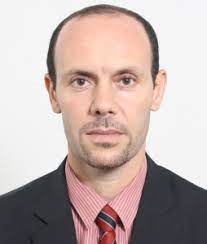
\includegraphics[width=2.5cm,height=4cm,clip,keepaspectratio]{a1}}]
\textbf{Saad Mekhilef} %% Affiliation and educational background.
\href{https://orcid.org/0000-0001-8544-8995}{
\includegraphics[width=0.02\textwidth]{orcid.png}} 
\href{https://scholar.google.co.id/citations?user=0kKMcLYAAAAJ&hl=en}{
\includegraphics[width=0.02\textwidth]{gscholar.png}}
\href{https://www.scopus.com/authid/detail.uri?authorId=6603317449}{
\includegraphics[width=0.02\textwidth]{scopus.png}}
\href{https://publons.com/researcher/1354246/mekhilef-saad/}{
\includegraphics[width=0.02\textwidth]{publons.png}} received the B.Eng. degree in electrical engineering from the University of Setif, Setif, Algeria, in 1995, and the master’s degree in engineering science and the Ph.D. degree in electrical engineering from the University of Malaya, Kuala Lumpur, Malaysia, in 1998 and 2003, respectively. He is currently a Professor and the Director of the Power Electronics and Renewable Energy Research Laboratory, Department of Electrical Engineering, University of Malaya, where he is also the Dean of the Faculty of Engineering. He is also a Distinguished Adjunct Professor with the School of Software and Electrical Engineering, Faculty of Science, Engineering and Technology, Swinburne University of Technology, VIC, Australia. His current research interests include power converter topologies, the control of power converters, renewable energy, and energy efficiency. He can be contacted at email: saad@um.edu.my.
\end{biography}

\begin{biography}[{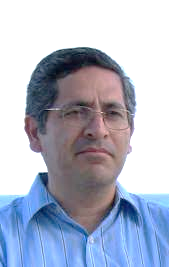
\includegraphics[width=2.5cm,height=4cm,clip,keepaspectratio]{a2}}]
\textbf{Oscar Castillo} %% Affiliation and educational background.
\href{https://orcid.org/0000-0002-7385-5689}{
\includegraphics[width=0.02\textwidth]{orcid.png}} 
\href{https://scholar.google.com/citations?user=1C8gb8IAAAAJ&hl=en}{
\includegraphics[width=0.02\textwidth]{gscholar.png}}
\href{https://www.scopus.com/authid/detail.uri?authorId=7007101709}{
\includegraphics[width=0.02\textwidth]{scopus.png}}
\href{https://publons.com/researcher/1331983/oscar-castillo/}{
\includegraphics[width=0.02\textwidth]{publons.png}} received the D.Sc. degree (Doctor Habilitatus) in computer science from the Polish Academy of Sciences, Warsaw, Poland, with the Dissertation “Soft Computing and Fractal Theory for Intelligent Manufacturing”. He is a Professor of computer science in the Graduate Division, Tijuana Institute of Technology, Tijuana, Mexico. In addition, he is serving as Research Director of computer science and Head of the research group on fuzzy logic and genetic algorithms. He is currently the Vice-President of Hispanic American Fuzzy Systems Association (HAFSA) and President Elect of International Fuzzy Systems Association (IFSA). He has published over 80 journal papers, 6 authored books, 20 edited books, and 200 papers in conference proceedings. His research interests are in Type-2 Fuzzy Logic, Fuzzy Control, Neuro-Fuzzy and Genetic-Fuzzy hybrid approaches. He can be contacted at email: ocastillo@tectijuana.mx.
\end{biography}

\begin{biography}[{
\includegraphics[width=2.5cm,height=4cm,clip,keepaspectratio]{a3}}]
\textbf{Patricia Melin} %% Affiliation and educational background.
\href{https://orcid.org/0000-0001-5798-1426}{
\includegraphics[width=0.02\textwidth]{orcid.png}} 
\href{https://scholar.google.com/citations?user=Ts6JtfMAAAAJ&hl=en}{
\includegraphics[width=0.02\textwidth]{gscholar.png}}
\href{https://www.scopus.com/authid/detail.uri?authorId=7006491873}{
\includegraphics[width=0.02\textwidth]{scopus.png}}
\href{https://publons.com/researcher/1332081/patricia-melin/}{
\includegraphics[width=0.02\textwidth]{publons.png}} received the D.Sc. degree (Doctor Habilitatus D.Sc.) in computer science from the Polish Academy of Sciences, Warsaw, Poland, with the Dissertation “Hybrid Intelligent Systems for Pattern Recognition using Soft Computing”. She is a Professor of Computer Science in the Graduate Division, Tijuana Institute of Technology, Tijuana, Mexico since 1998. In addition, she is serving as Director of Graduate Studies in computer science and Head of the research group on Computational Intelligence (2000–present). Her research interests are in Type-2 Fuzzy Logic, Modular Neural Networks, Pattern Recognition, Neuro-Fuzzy and Genetic-Fuzzy hybrid approaches., She is currently the President of Hispanic American Fuzzy Systems Association (HAFSA) and is the founding Chair of the Mexican Chapter of the IEEE Computational Intelligence Society. She can be contacted at email: pmelin@tectijuana.mx.
\end{biography}


\end{document}

%%
%% End of file `telkomnika.tex'. 